\documentclass[aps,rmp, onecolumn]{revtex4}
%\documentclass[a4paper,10pt]{scrartcl}
%\documentclass[aps,rmp,twocolumn]{revtex4}

\usepackage[utf8]{inputenc}
\usepackage{amsmath,graphicx}
\usepackage{color}
%\usepackage{cite}

\newcommand{\bq}{\begin{equation}}
\newcommand{\eq}{\end{equation}}
\newcommand{\bn}{\begin{eqnarray}}
\newcommand{\en}{\end{eqnarray}}
\newcommand{\Richard}[1]{{\color{red}Richard: #1}}
\newcommand{\gene}[1]{{\it #1}}
\newcommand{\mat}[1]{{\bf #1}}
\newcommand{\vecb}[1]{{\bf #1}}
\newcommand{\abet}{\mathcal{A}}
\newcommand{\eqp}{p}
\newcommand{\LH}{\mathcal{L}}

\bibliography{bib}

\begin{document}
\title{Evolutionary rates of SARS-CoV-2}
\author{Richard A.~Neher}
\date{\today}
\maketitle

Since its emergence in late 2019, SARS-CoV-2 has displayed a discontinuous pattern of evolution with large unobserved jumps in sequence space giving rise to new variants \citep{alpha,beta,gamma,delta,omicron}.
\begin{itemize}
    \item hypothesis of the jumps
    \item link to other examples of decaying rate of evolution H1N1pdm, HIV within host
    \item
\end{itemize}

Traditionally, evolutionary rates and divergence times are estimates using phylogenetic frameworks for heterochronously sampled sequences.
The volume and heterogeneity of SARS-CoV-2 data, however, mean that one has to dramatically down-sample the data and remove many low quality sequences that would otherwise fatally distort the analysis.


To circumvent many of the above mentioned problems and still use the majority of the available data, we use a combination of automated filtering and robust procedures to analyze the evolutionary patterns.
We first use Nextclade \citep{aksamentov_nextclade_2021} to assign all sequences to one of the Nextstrain \citep{hadfield_nextstrain_2018} clades and analyze each clade separately.
These clades represent well defined groups of sequences with little non-vertical evolution within them.
Furthermore, we define a ``founder'' genotype for each clade and exclude any sequence that does not have the full set of mutations relative to the reference sequence Wuhan/Hu-1.
This filtering removes most incomplete sequences as well as sequences where amplicon drop-out are back-filled with reference sequence.
For this reduced set of sequences, we determine the mutations they carry on top of the founder genotype.
The latter step is done for nucleotide changes as well as for amino acid changes.

Within each clade, the number of mutations is expected to increase linearly in time and the variation around this mean would, in an ideal case, obey Poisson statistics.
To further exclude outliers, we perform a simple linear regression of the number of ``intra-clade'' mutations against time and remove sequences whose deviation from the linear fit exceeds twice the variance by 3.

After removing these outliers, we now bin the data by calendar week and determine the mean and standard deviation in each bin.
Evolutionary rate and putative emergence date of the variant are then estimated by weighted linear regression where each bin is weighted with the fourth root of the number of sequences in the bins.
The exact functional form of this weighing does not have a big influence on the results, but a strongly sublinear weighing helps to counter the large variation in sequencing effort and the natural imbalance due to the fact that few sequences are available early.

Due to shared ancestry, a divergence (or root-to-tip) regression against time is not a suitable method to determine the evolutionary rate.
However, in the case of rapidly expanding variants we typically observe a large number of independent lineages emanating from a basal polytomy.
Along each of these lineages, mutation accumulation is independent.
\begin{figure*}
    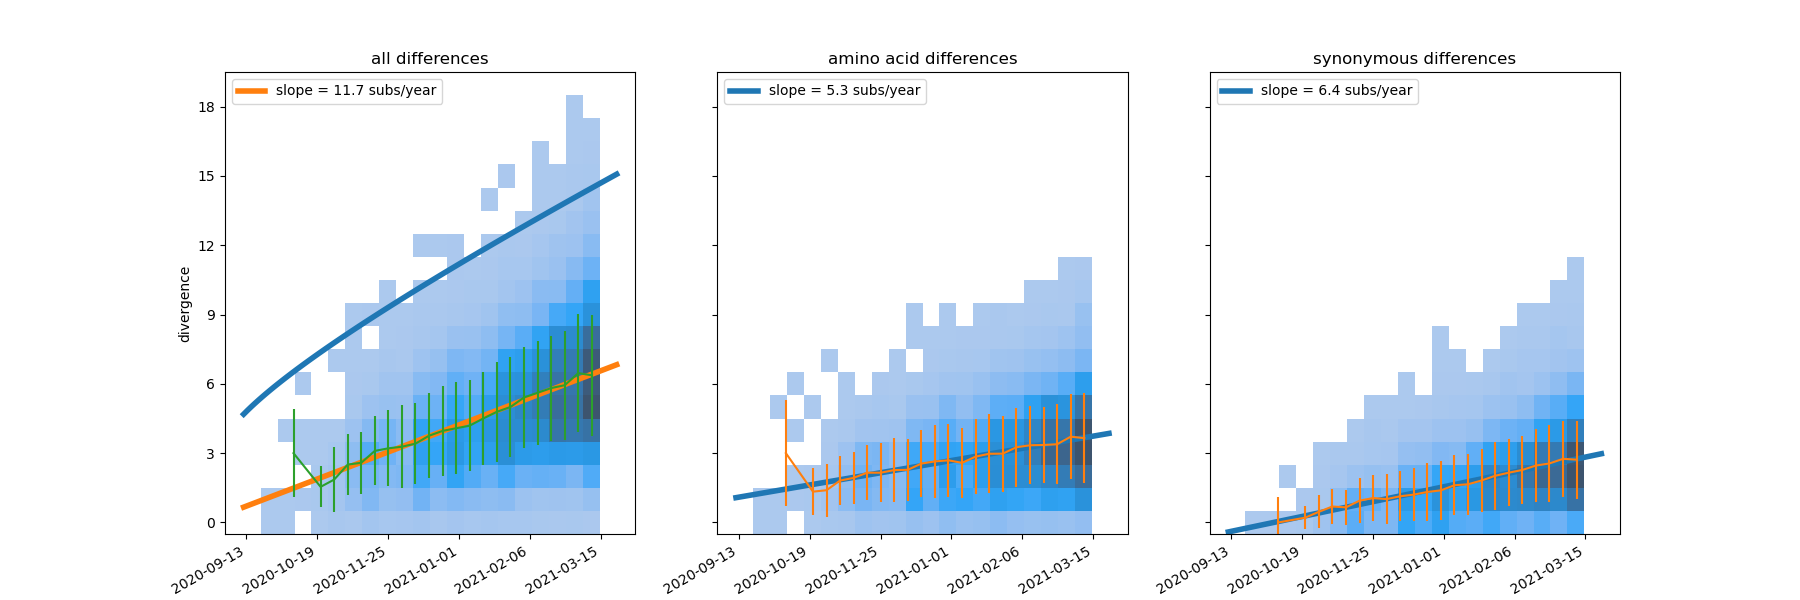
\includegraphics[width=\textwidth]{figures/20I_rtt.png}
    \caption{{\bf Divergence increases linearly with time (20I (Alpha)).} Each panel shows the number of within-clade mutations (total (A), amino acid changing (B), synonymous (C)) as a function of time.
    The blue line in panel A indicates the divergence cut-off, panels B\&C only show sequences that pass the divergence filter. Each panel also shows mean $\pm$ standard deviation and a weighted linear fit.}
\end{figure*}




\end{document}
